\def\year{2019}\relax
%File: formatting-instruction.tex
\documentclass[letterpaper]{article} %DO NOT CHANGE THIS
\usepackage{aaai19}  %Required
\usepackage{times}  %Required
\usepackage{helvet}  %Required
\usepackage{courier}  %Required
\usepackage{url}  %Required
\usepackage{graphicx}  %Required
\frenchspacing  %Required
\setlength{\pdfpagewidth}{8.5in}  %Required
\setlength{\pdfpageheight}{11in}  %Required
%PDF Info Is Required:
  \pdfinfo{
/Title (2019 Formatting Instructions for Authors Using LaTeX)
/Author (AAAI Press Staff)}
\usepackage{algorithm,amsmath}
\usepackage{algorithm}
\usepackage{algorithmic}
\usepackage{mathtools}
\usepackage{newtxtext,newtxmath}
\usepackage[tight,footnotesize]{subfigure}
\let\openbox\relax
\usepackage{amsthm}
\usepackage[dvipsnames]{xcolor}
\newcommand*{\R}{\mathbb{R}}
\newcommand*{\Po}{\text{Prox}}
\newcommand*{\Am}{\text{argmin}}
\newcommand*{\E}{\mathbb{E}}
\newcommand*{\VRG}{\,\tilde{\nabla}_k^s}
\newcommand{\norm}[1]{\left\lVert#1\right\rVert}
\newcommand{\Iprod}[2]{\left\langle #1,#2\right\rangle}
\newcommand\myeq[2]{\mathrel{\stackrel{{{#1}}}{#2}}}

\renewcommand{\algorithmicrequire}{
\textbf{Input:}}
\renewcommand{\algorithmicensure}{\textbf{Output:}}
\newcommand{\Initialize}{\textbf{Initialize:}{\,}}
\newcommand{\Input}{\textbf{Input:}{\,}}
\newcommand{\Output}{\textbf{Output:}{\,}}


\newtheorem{theorem}{Theorem}
\newtheorem{lemma}{Lemma}
\newtheorem{conjecture}[theorem]{Conjecture}
\newtheorem{condition}[theorem]{Condition}
\newtheorem{claim}[theorem]{Claim}
\newtheorem{question}[theorem]{Question}
\newtheorem{corollary}{Corollary} 
\newtheorem{definition}{Definition}
\newtheorem{statement}[theorem]{Statement}
\newtheorem{notation}[theorem]{Notation} 
\newtheorem{remark}{Remark}
\newtheorem{Assumption}{Assumption}
\setcounter{secnumdepth}{0}  
 \begin{document}
% The file aaai.sty is the style file for AAAI Press 
% proceedings, working notes, and technical reports.
%
\title{Distributed Accelerated Proximal Optimization Algorithms with Variance Reduction
}
\maketitle

\begin{abstract}
    The proximal stochastic gradient descent (ProxSGD) has been widely used to solve composite convex optimization problems. However, the random sampling in ProxSGD introduces noisy gradient updates with high variance, which causes to use a vanishing step size and so slows down the convergence as the iterates approach the optimum.  In addition, although ProxSGD with variance-reduction enjoys great success in applications at small and moderate scales, but distributed versions of these algorithms are crucially demanded for larger-scale training datasets. In this paper, we propose a synchronous method, Sync-AcPSVRG, and an asynchronous method, Async-AcPSVRG, which integrate variance-reduction and momentum acceleration techniques in a distributed manner. To the best of our knowledge, this paper provides one of the first analysis of distributed accelerated ProxSGD that can achieve significant speedup with the number of workers without hurting the convergence rate. Both Sync-AcPSVRG and Async-AcPSVRG enjoy lower iteration  complexity than existing  accelerated  stochastic  variance  reduction  methods, which need more updates per iteration. Furthermore, we allow the number of updates to increase with the epochs to secure sparse communications between workers and master. We compare distributed AcPSVRG with existing parallel stochastic proximal optimization methods on a few datasets. The empirical results verify our theoretical results and indicate that our proposed distributed accelerated methods with variance reduction have significant superiority  than other ProxSGD variants.
\end{abstract}
%\begin{IEEEkeywords}

%\end{IEEEkeywords}

\section{Introduction}

In this paper, we consider the following composite optimization problem 
\begin{equation}\label{problem}
    \min_{x\in\R^d}\,F(x) = h(x) + f(x)= h(x) + \frac{1}{n} \sum_{i=1}^n f_i(x),
\end{equation}
where $f_i(x)$, $i=1,2,\ldots,n$, are smooth convex loss functions, and $h(x)$ is a non-smooth regularization term. Proximal stochastic gradient descent (ProxSGD) \cite{Nemirovski2009} is a general approach for solving minimization problem in \eqref{problem}, which employs the fact that the objective function decomposes into a sum over many terms. 

For problems where each $f_i$ in \eqref{problem} corresponds to a single data observation, ProxSGD selects a single data index $i_k$ on each iteration $k$, and then performs update by solving the proximal optimization subproblem
\[
x^{k+1} = \Po_{\eta, h}\{x^{k} -\eta \nabla f_{i_k} (x_k)\},
\]
where the proximal mapping is defined as 
\[
\Po_{\eta,h}(y) = \displaystyle{\text{ argmin}}_{x\in\R^d}\{\frac{1}{2\eta}\norm{x-y}^2+h(x)\}.
\]
In the above notation $\norm{\cdot}$ is the $L_2$-norm and $\eta$ is the step size.
Typically, $i_k$ is chosen uniformly at random from $\{1, 2,\ldots, n\}$ on each iteration $k$, thus making the gradient approximation unbiased. However, because random sampling in ProxSGD introduces variance, vanishing step sizes are needed to guarantee the algorithm's convergence,
and the convergence rate is only sublinear \cite{Langford2009,rakhlin2012making}. In \cite{Xiao2014}, a variance reduction technique for proximal algorithms was introduced and it is proved that it can achieve linear convergence. The convergence rate of ProxSGD with variance reduction can be further improved with the so-called momentum acceleration technique \cite{Allen-Zhu17}.

Another major drawback of ProxSGD is the sequential nature of algorithm. For massive datasets or training datasets distributed over a cluster of multiple nodes, parallel or distributed algorithms are sorely needed, making more practical impacts on parallel SGD variants to solve large-scale or distributed problems. There is quite a bit of recent works in the area of distributed optimization that have been successfully applied to accelerate many optimization algorithms including SGD \cite{Agarwal2014,Recht2011,Mania2017} and ProxSGD \cite{LiP2016,Meng2017}.   

In this paper, we propose distributed algorithms to enhance the scalability of proximal algorithms using variance reduction and momentum acceleration techniques, yielding ProxSGD methods that scale near linearly and can provide better convergence rate.

\section{Backgrounds}
Since SGD estimates the gradient from only one or a few samples, the variance of the stochastic gradient estimator may be large \cite{Johnson12,Zhao2015}, which leads to slowdown and poor performance. Recently there has been a lot of interest in methods which reduce the variance incurred due to stochastic
gradients. Variance reduction (VR) methods \cite{Johnson12,Defazio2014} reduce the variance in the stochastic gradient estimates, and are able to alleviate the effects of vanishing step sizes that usually hit SGD, and yield methods that improve convergence rates both theoretically and empirically. 
Inspired by the success of these methods in reducing the gradient noise in stochastic gradient based optimization, recently many variants of variance reduction methods have been proposed \cite{Konecny2016,Li2016,Xiao2014,Allen-Zhu2016,shang2018guaranteed}. Variance reduction methods begin with an initial estimate $\widetilde{x}$, and then generate a sequence of iterates $x_k$ from
\[x_k = x_{k-1} - \eta\left[\nabla f_{i_k}(x_{k-1})-\nabla f_{i_k}(\widetilde{x}) + \widetilde{\nabla}f(\widetilde{x})\right],
\]
where $\eta$ is the step size, $\widetilde{\nabla}f(\widetilde{x})$ is an approximation of the true gradient, and $\widetilde{x}$ is chosen to be a recent iterate from algorithm history. In particular, an error correction term is subtracted from regular update rules in stochastic optimization to reduce the variance of gradients in order to deal with the problems of instability and slower convergence hit SGD.


Recently several acceleration techniques based on momentum compensations were introduced to further speed up the VR methods mentioned above \cite{Hu2009,Lin2015,nitanda2014,Allen-Zhu17}. The momentum acceleration technique, which is basically proposed by Nesterov \cite{Nesterov2004} for gradient methods, introduces one or multiple auxiliary variables to record the momentum, and updates the parameters according to the gradient at the auxiliary variable. To be specific, with momentum acceleration, the update rule becomes
\begin{equation}
\begin{split}
x_{k+1}& = z_k-\eta \nabla f_{i_k}(z_k),\\
z_{k+1}& = x_{k+1} + \beta (x_{k+1}-x_{k}),
\end{split}
\end{equation}
where $\beta$ is the momentum weight. It can be proven that the convergence rate of SGD
is improved by using the Nesterov acceleration technique \cite{Hu2009}.
After that, many accelerated algorithms have been designed to achieve faster convergence rates for stochastic optimization methods \cite{Shalev-Shwartz2014,Allen-Zhu17,Fercoq2015,Lin2015}.

Although these acceleration techniques have great value in general, for large-scale problems, however, with the availability of very big training data, sequential SGD is very inefficient. Therefore, integrating the VR algorithms and acceleration techniques to distributed settings remain indispensable. In \cite{Reddi2015,Mania2017} SVRG is extended to the parallel asynchronous setting. In particular, in \cite{Meng2016} a parallel algorithm mitigated by variance reduction, coordinate sampling, and Nesterov's method is introduced. But the scalability of this algorithm is only proven for sparse datasets and under appropriate parameter setting. An asynchronous implementation of VR method with acceleration is presented in \cite{fang2018accelerating}, however it requires learning rate to decrease with the square  of the upper bound for delays, i.e. $\tau^2$, and thereby an asynchronous speedup is not shown. In addition, their algorithm design requires at least two auxiliary variables
and two momentum parameters, which makes it difficult to store and process on local nodes, and increases the  complexity per iterations. 


In this paper, we introduce distributed synchronous and asynchronous SGD-based algorithms with variance reduction integrated with acceleration techniques, which have not been well studied in the literature to the best of our knowledge. We prove that the proposed distributed algorithms have desirable convergence property, show considerable speedup. The parallel algorithms are highly scalable, uses a constant learning rate for convex functions, and converges linearly to the optimal solution in the strongly convex case.

\section{Our Approaches}
In this work, we attempt to introduce momentum to accelerate distributed variance reduction SGD algorithms for convex problems. We demonstrate that one step of momentum with only one weight provides a faster convergence rate in expectation, while we assume an upper bound for delay $\tau$ between delayed gradient and the latest one. 

By applying this technique in distributed stochastic algorithms, we allow many local nodes to run simultaneously, while communicating 
with the server node through the exchange of updates. This new algorithm allows many processes to work towards a central solution which are
faster by order than existing variance-reduced ProxSGD algorithms. 

This work has three main contributions:

\begin{enumerate}
    
\item We propose distributed algorithms for convex problems adopted with variance reduction methods and momentum acceleration techniques with only one momentum weight. The space requirement of the proposed algorithms is advantageous compared to the existing accelerated stochastic variance reduction methods, e.g., \cite{Allen-Zhu17,fang2018accelerating}, in that they only need to store one additional variable for the momentum term. In our asynchronous  algorithm, local nodes only need to store the averaged sample gradient which is more suitable for optimization with a
large number of variables. 

\item We theoretically study the convergence for general proximal algorithm and obtain improved convergence rate for convex and strongly convex functions. We will show our proposed distributed algorithms with acceleration and variance reduction, can speed up on sparse or dense data. It is scalable and uses a constant learning rate for convex functions. To the best of our knowledge it is the first analyses to achieve speedup with no assumptions on sparsity and the number of workers. The algorithms uses a constant learning rate for convex functions and the learning rate has to decrease only with $\tau$. 
 
\item Finally, we present several empirical results over several distributed VR algorithms to demonstrate that the new accelerated algorithm 
can lead to better performance improvements and promising speedup than competing options, which agrees with our theory. 
\end{enumerate}

\section{{Algorithm Overview}}

We begin by proposing our new accelerated proximal variance reduction scheme with momentum acceleration (AcPSVRG), in the single-worker case. 
As we will see later, the proposed method has a natural generalization to the distributed setting that has low communication requirement. Similar to the epoch gradient descent algorithm \cite{Hazan2011}, we increase the number of iterations by a constant $\gamma$ for every epoch. 

Our proposed VR scheme (AcPSVRG) is divided into $S$ epochs, with $m_s$ updates taking place in each epoch.  Throughout the paper, we will
use the superscript for the index of each epoch, and the subscript for the index of iterations within each epoch.

Let the iterates generated in the $s$-th epoch be written as $\{x_k^s\}_{k=0}^{m_s-1}$. The update rule for AcPSVRG can be formulated as follows: 

In each iteration the following type of proximal subproblem is solved,
\begin{equation}
z_{k+1}^s = \Po_{\frac{\eta}{\beta_s}} h \{z_{k}^s - \frac{\eta}{\beta_s}\widetilde{\nabla}_k^s\},
\end{equation}
where
\begin{equation}\label{nabla-update}
\widetilde{\nabla}_k^s = \nabla f_{i_k^s}(x_k^s) - \nabla f_{i_k^s}(\widetilde{x}^{s-1}) + \nabla f(\widetilde{x}^{s-1}).
\end{equation}
We let snapshot $\widetilde{x}^s$ be a weighted average of $x_k^{s}$ in the most recent epoch $s$, which is updated at the end of each epoch, i.e., after every $m_s$ parameter updates. We compensate the momentum term and introduce a new extrapolation rule to update $x_k^{s}$,
\[
x_{k+1}^s = \widetilde{x}^s+\beta_s(z_{k+1}^s-\widetilde{x}^s),
\]
where $\beta_s \in [0, 1]$ is the momentum weight. Indeed, $z_{k+1}^s$ is a momentum which adds a weighted sum of gradient history into $x_k^{s}$. Comparably, this update has only one momentum weight $\beta_s$ versus two weights $\tau_1$ and $\tau_2$ in \cite{Allen-Zhu17} through introducing two momentum vectors.  
We increase the number of
iterations by a constant $\gamma$ for every epoch, i.e., $m_{s+1} = \gamma m_{s}$.
The choice of growing the iterations per epoch can reduce the number of full gradient calculations and the frequency of communication between
the server and the local nodes in the distributed setting, while it can speed up the convergence \cite{Allen-Zhu2016I}.

Note that if $i_k^s$ in \eqref{nabla-update} is chosen uniformly at random from the set $\{1,2,\ldots,n\}$ on each iteration $k$, then, conditioning on all history,
\[
\E[\nabla f_{i_k^s}(\widetilde{x})] = \nabla f(\widetilde{x}).
\] 
Thus, the error correction term has expected value $0$, and $\E[\widetilde{\nabla}_k^s] = \nabla f(x_{k}^s)$, i.e., the approximate gradient $\widetilde{\nabla}_k^s$ is unbiased.

\section{Distributed Algorithms}

We now consider the distributed setting, on a master-slave framework with a master machine and $p$ local clients, each of which contains a portion of
the data set. In this setting, the whole data $\Omega$ is decomposed into disjoint
subsets $\{\Omega_k\}$,  where $k$ denotes  a  particular  local  worker,
and $\cup_{l=1}^p{\Omega_l} = \Omega$ and if $i\neq j$, $\Omega_i\cap\Omega_j = \emptyset$. Different clients can not communicate with each other and the  clients  can
only communicate with the central server. Our model of
computation is similar to the ones used in Parameter
Server \cite{Li2014} and Mllib \cite{Meng2016Spark}. Our goal is to
derive stochastic algorithms that scale linearly to high $p$.

\subsection{Synchronous Accelerated SGD}

AcPSVRG naturally extends to the distributed synchronous
setting,  and  is  presented  in  Algorithm  \ref{SyncVR-Algo-Single}.  To  distinguish  the
algorithm from the single worker case, we call it Sync-AcPSVRG. 
\begin{algorithm}[H]
\caption{Sync-AcPSVRG}\label{SyncVR-Algo-Single}
\begin{algorithmic}
\renewcommand{\algorithmicrequire}{\textbf{Input:}}
 \renewcommand{\algorithmicensure}{\textbf{Output:}}
  \newcommand{\INITIALIZE}{\item[\textbf{Initialize:}]}
\REQUIRE The number of epochs $S$ and the step size $\eta$
\INITIALIZE $\widetilde{x}^0$, $m_1$, $\theta_1$, and $\rho > 1$
\FOR {{\bf Worker} $l$} 
\FOR{ $s=1$ {\bf to} $S$ }
\STATE Receive $\widetilde{x} = \widetilde{x}^{s-1}$ from master node.
\STATE  Send $\nabla_l f(\widetilde{x}) = \sum_{i\in\Omega_l}\nabla f_i(\widetilde{x})$ to master node.
\STATE  Receive $\nabla f(\widetilde{x})$ from master node.
 \STATE $x_{l,0}^s = z_{l,0}^s = \widetilde{x}$
 \FOR{$k=0$ {\bf to} $m_s-1$}
 \STATE Pick $i_{l,k}^s$ uniformly at random from $\Omega_l$.
 \STATE $\widetilde{\nabla}_{l,k}^s = \nabla f_{i_{l,k}^s}(x_{l,k}^s) - \nabla f_{i_{l,k}^s}(\widetilde{x}) + \nabla f(\widetilde{x})$
 \STATE $\delta_{l,k}^s = \text{argmin}_{\delta}\,\,h(z_{l,k}^s+\delta)+\langle\widetilde{\nabla}_{l,k}^s,\delta\rangle + \frac{{\beta_s}}{2\eta}\norm{\delta}^2$
 \STATE $z_{l,k+1}^s = z_{l,k}^s + \delta_{l,k}^s$
 \STATE $x_{l,k+1}^s = \widetilde{x}+\beta_s(z_{l,k+1}^s-\widetilde{x})$
 \ENDFOR
\STATE $\widetilde{x}_{l}^s = \frac{1}{m_s}\sum_{k=0}^{m_s-1} x_{l,k}^s$, $m_{s+1} = \gamma m_s$
\STATE Send $\widetilde{x}_{l}^s$ to master node.
 \ENDFOR
 \ENDFOR
 \STATE{\bf Master Node:}
 \STATE\qquad\,\,\,\, Average $\widetilde{x}_l$ received from workers.
  \STATE\qquad\,\,\,\, Broadcast averaged $\widetilde{x}$ to local workers.
  \STATE\qquad\,\,\,\, Average $\nabla f(\widetilde{x}_l)$ received from workers.
  \STATE\qquad\,\,\,\, Broadcast averaged $\nabla f(\widetilde{x})$ to local workers.
 \ENSURE $\widetilde{x}^S$
\end{algorithmic}
\end{algorithm}
{Note, the number of updates per epoch $m_s$ and $\widetilde{x}^s$ are initialized with $m_1$ and $\widetilde{x}^0$. At the beginning of each epoch we initialize $x_0^s=z_0^s=\widetilde{x}^{s-1}$, where $\widetilde{x}^{s-1}$ is the average of the past $m_{s-1}$ stochastic iterations.} On  each  epoch,  the  local  nodes  first  retrieve  a  copy of  the  central  iterate $\widetilde{x}^{s-1}$, compute the sum of the gradients on its local data, i.e., $\sum_{i\in\Omega_k}{\nabla f_i{(\widetilde{x}^{s-1})}}$ and send it to the master node. The accelerated VR method is then locally performed on each node by only using the local data, and each worker sends the most recent parameter denoted as ${x}_k$ for $k$-th worker to the master. Then parameter $\widetilde{x}^s$ is updated by the master after all the locally updated parameters have been gathered. As we put now constraint on how training data are partitioned on different workers, by sharing full gradient $\nabla f(\widetilde{x})$ across nodes, we ensure  that  the  local  gradient  updates  utilize  global  gradient information from remote nodes. We ensure also local updates are not far away from global updates through including momentum. This speeds up the convergence of stochastic optimization and controls the difference between the local update and global update, even if each local  node  runs  for  one  whole  epoch  before  communicating back with the central node. 

In Sync-AcPSVRG, as we mentioned earlier, we assume that each worker has access to a subset and not the entire data set and performs local updates for one epoch, or iterations, before communicating with
the  server. This  is  a  rather  low  communication  frequency
compared  to  a mini-batch parameter  server  model such as parallel implementation of SVRG \cite{Zhao2014} or mS2GD \cite{Konecny2016} in which stochastic optimization is performed on the master node based on the whole dataset, and updates and gradients are frequently transferred between workers and master. This  makes  a  significant  difference  in  runtimes  when  the
number of local nodes is large.
 We also increase the number of inner updates per epoch by a constant $\gamma$ which reduces the communication rate between server and worker because there is no communication during the inner iterations of each epoch and yields fastest convergence. We also let local workers make updates according to the proximal solver.

\subsection{Asynchronous Accelerated SGD}

The  synchronous algorithm could be extended to the asynchronous one called Async-AcPSVRG  as shown in Algorithm \ref{AsyncVR-Algo}. We adopt asynchronous update in each inner loop and there is synchronization operation after each epoch. In Async-AcPSVRG, the  master node keeps a copy of the averaged $x$. We make workers do proximal mapping step, and server is responsible for element-wise addition operations, perform a momentum update, average $x$, aggregate full gradient and then broadcast it to workers at the end of each epoch. 
The key idea for Async-AcPSVRG is that, once a local node solves the proximal update, it  sends  the update to the master. The master thread will use the update received by the local node to update $x$. Each processor repeatedly runs these procedures concurrently, without any synchronization. We use $k-\tau_k$ to denote the state of $x$ at the reading time by the local worker. For asynchronous algorithms, the partial gradient calculated by the local worker will be delayed, and at iteration $k$ the worker $l$ could only obtain $\nabla f_{i_{l,k}^s}(x_{k-\tau_k}^s)$ instead of $\nabla f_{i_{l,k}^s}(x_{k}^s)$. We assume that the delay between the time of evaluation and updating is bounded by a non-negative integer $\tau$, i.e., $\tau_k\leq \tau$. The parameter $\tau$ captures the degree of delay. When there are more threads, the delay accumulates and results in larger $\tau$. Furthermore, we also assume that the system is synchronized after every epoch.

For the purpose of our analysis, we assume a consistent read model, i.e., when $x$ is read or updated in the central node, it will be locked. However, the proposed asynchronous algorithms can be easily implemented in a lock-free setting, leading to further speedups. We leave the analysis of inconsistent read (wild) model as future work.
\begin{algorithm}[H]
\caption{Async-AcPSVRG}\label{AsyncVR-Algo}
\begin{algorithmic}
\renewcommand{\algorithmicrequire}{\textbf{Input:}}
 \renewcommand{\algorithmicensure}{\textbf{Output:}}
  \newcommand{\INITIALIZE}{\item[\textbf{Initialize:}]}
\REQUIRE The number of epochs $S$ and the step size $\eta$.
\INITIALIZE  $\widetilde{x}^0$, $m_1$, $\theta_1$, and $\rho > 1$

\FOR{ $s=1$ to $S$ }
\STATE $t=0$;
\STATE{\bf Worker $l$} 
\STATE Wait until it receives $\widetilde{x} = \widetilde{x}^{s-1}$ from master node.
\STATE  Send $\nabla_l f(\widetilde{x}) = \sum_{i\in\Omega_l}\nabla f_i(\widetilde{x})$ to master node.
\STATE  Wait until it receives $\nabla f(\widetilde{x})$ from master node.
\STATE $x_{l,0}^s = z_{l,0}^s = \widetilde{x}$
 \FOR{$k=0$ to $m_s-1$}
 \STATE Receive $x_{l,k-\tau_k}^s:=x_{t}^s$ from master node.
 \STATE Pick $i_{l,k}^s$ uniformly at random from $\Omega_l$.
 \STATE $\widetilde{\nabla}_{l,k}^s = \nabla f_{i_{l,k}^s}(x_{l,k-\tau_k}^s) - \nabla f_{i_{l,k}^s}(\widetilde{x}) + \nabla f(\widetilde{x})$
 \STATE $\delta_{l,k}^s = \text{argmin}_{\delta}\,\,h(z_{l,k}^s+\delta)+\langle\widetilde{\nabla}_{l,k}^s,\delta\rangle + \frac{{\beta_s}}{2\eta}\norm{\delta}^2$
 \STATE $z_{l,k+1}^s = z_{l,k}^s + \delta_{l,k}^s$
 \STATE Send $z_{l,k+1}^s$ to master node.
\STATE{\bf Master Node:}
 \STATE Receive $z_{l,k+1}^s$ from worker $l$. 
  \STATE Update $x^s_{t+1} = \widetilde{x}+\beta_s(z_{l,k+1}^s-\widetilde{x})$, $t=t+1$.
  \ENDFOR
  \STATE {\bf Master Node:}
   \STATE Calculate average $\widetilde{x}^s = \frac{1}{t}\sum_{i=1}^{t} x_{i}^s$ and broadcast averaged $\widetilde{x}^s$. 
  \STATE Receive $\nabla_l f(\widetilde{x}^s)$ from workers and calculate average $\nabla f(\widetilde{x}^s)$.
  \STATE Broadcast averaged $\nabla f(\widetilde{x}^s)$ to local workers.
  \STATE $m_{s+1} = \gamma m_s$
  \ENDFOR
 \ENSURE $\widetilde{x}^S$
\end{algorithmic}
\end{algorithm}

\section{Convergence Analysis}
In this section, we provide convergence analysis for distributed AcPSVRG. For further analysis, throughout this paper, we make the following assumptions, which are commonly used in previous works \cite{Reddi2015,Meng2016}.

\begin{Assumption}[Lipschitz Gradient]\label{Assump1}
The components $f_i(x), i=1,2,\ldots,n$ are differentiable and have Lipschitz continuous partial gradients, i.e., for $x,y\in \R^d$, we have,
\begin{equation}
    \norm{\nabla f_i(x) - \nabla f_i(y)} \leq L \norm{x-y}.
\end{equation}
\end{Assumption}
\begin{Assumption}[Convexity]\label{Assump2}
The components $f_i(x), i=1,2,\ldots,n$ and function $h(x)$ are convex. The objective function $F(x)$ could be strongly convex with parameter $\mu$, i.e., 
$\forall x,y \in \R^d$
\begin{equation}\label{Convex:Eq1}
F(y)\geq F(x) + \Iprod{\xi}{y-x} + \frac{\mu}{2}\norm{x-y}^2,\qquad \forall \xi\in\partial F(x),
\end{equation}
and for non-strongly convex functions $\mu=0$. 
\end{Assumption}

\begin{Assumption}[Bounded Delay]\label{Assump3}
The delays $\tau_1,\tau_2,\ldots$ are independent random variables, and $\tau_k\leq \tau$ for all $k$. As we mentioned earlier, we use $k-\tau_k$ to denote the read state at iteration $k$ in the asynchronous algorithm.
\end{Assumption}

Let $p(w)$ be a convex function over a convex set $X$. Let $\hat{w} = \text{argmin}_{w\in X}\{p(w)+\alpha\norm{w-\overline{y}}^2\}$ for some $\overline{y}\in X$ and $\alpha\geq 0$. Due to the fact that the sum of a convex and a strongly convex function is also strongly convex,  we have
\begin{equation}\label{threepoint-convex}
 p(w)+\alpha\norm{w-\overline{y}}^2 \geq p(\hat{w})+\alpha\norm{\hat{w}-\overline{y}}^2+\alpha\norm{w-\hat{w}}^2.
\end{equation}


\begin{lemma}\label{lemma0}\cite{Johnson12,Allen-Zhu17} If $f_i(x)$, $i=1,2,\ldots,n$ have $L$-Lipschitz continuous gradients, then with defining 
\[
\widetilde{\nabla} f(w) = \nabla f_k(w) - \nabla f_k(\widetilde{x})+ \nabla f(\widetilde{x}),
\]
we have
\begin{equation}
\begin{split}
\E&\left(\norm{\widetilde{\nabla} f(w)-\nabla f(w)}^2\right)\\
&~~~\leq 2L (f(\widetilde{x})-f(w)+\Iprod{\nabla f(w)}{w-\widetilde{x}}).
\end{split}
\end{equation}
\end{lemma}

\begin{lemma}\label{lemma1}
Under Assumptions \ref{Assump1}-\ref{Assump3}, if $x^*$ is the optimal solution of Problem \eqref{problem}, for the Algorithm \ref{AsyncVR-Algo} and $\eta < \min\{\frac{1}{4L
\tau}, \frac{1}{3L}\}$, we have 

\begin{equation}
\begin{split}
\E\left[ F(\widetilde{x}^s)\right. &-\left. F(x^*)\right]
\leq \lambda_s\E[F(\widetilde{x}^{s-1}) - F(x^*)]\\
&~~~+{\frac{\beta_s^2}{2\eta m_s(1-\alpha_s)}}\E[\norm{z_{0}^s-x^*}^2-\norm{z_{m_s}^s-x^*}^2 ],
\end{split}
\end{equation}
with $\lambda_s = \frac{(1-\beta_s+\alpha_s)}{1-\alpha_s}$, $\alpha_s=\frac{4(2+\theta_{\eta}^{-1})L^2\tau^2\eta^2}{1-2L^2 \tau^2\eta^2}$, $\theta_{\eta} = \frac{1-\eta L}{2\eta L}$ and $\beta_s$ is chosen such that $\beta_s < 1-\theta_{\eta}^{-1}$.
\end{lemma}
\begin{figure*}[htbp]
\subfigure[speedup on ijcnn]{
\centering
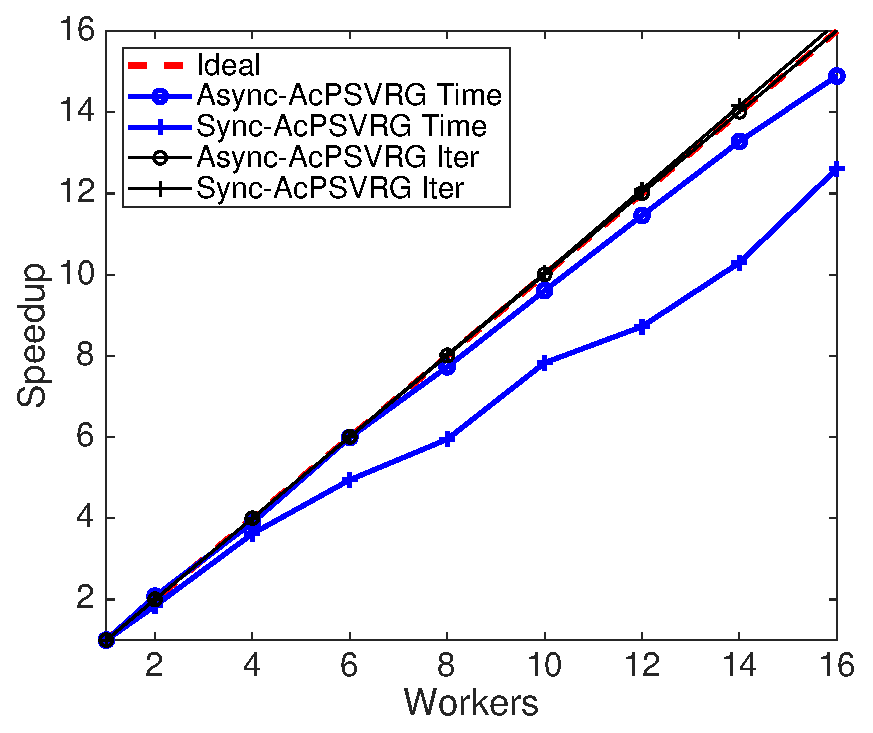
\includegraphics[width=0.24\linewidth]{../Figures/ijcnn_speedup_FSVRG.eps}}%
\subfigure[speedup on covtype]{
\centering
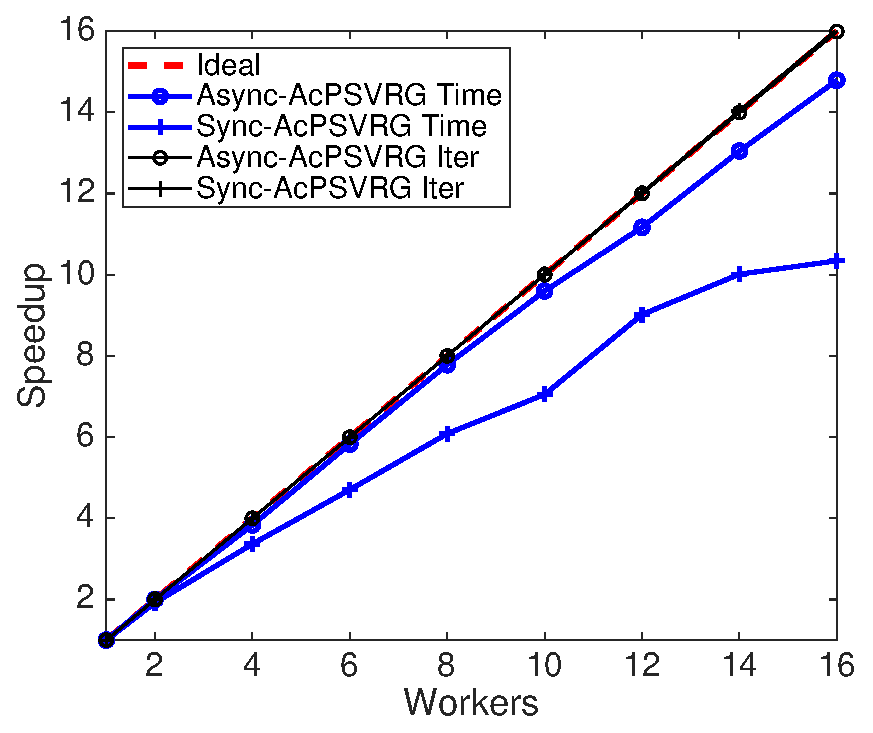
\includegraphics[width=0.24\linewidth]{../Figures/covtype_speedup_FSVRG.eps}}%
\subfigure[speedup on real-sim]{
\centering
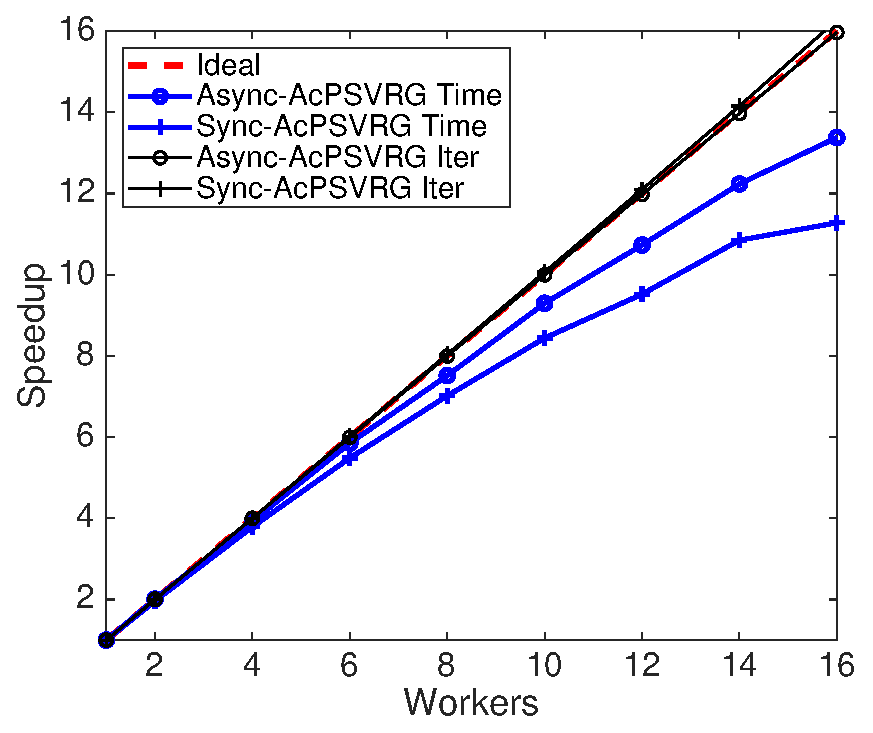
\includegraphics[width=0.24\linewidth]{../Figures/real-sim_speedup_FSVRG.eps}}%
\subfigure[speedup on rcv1]{
\centering
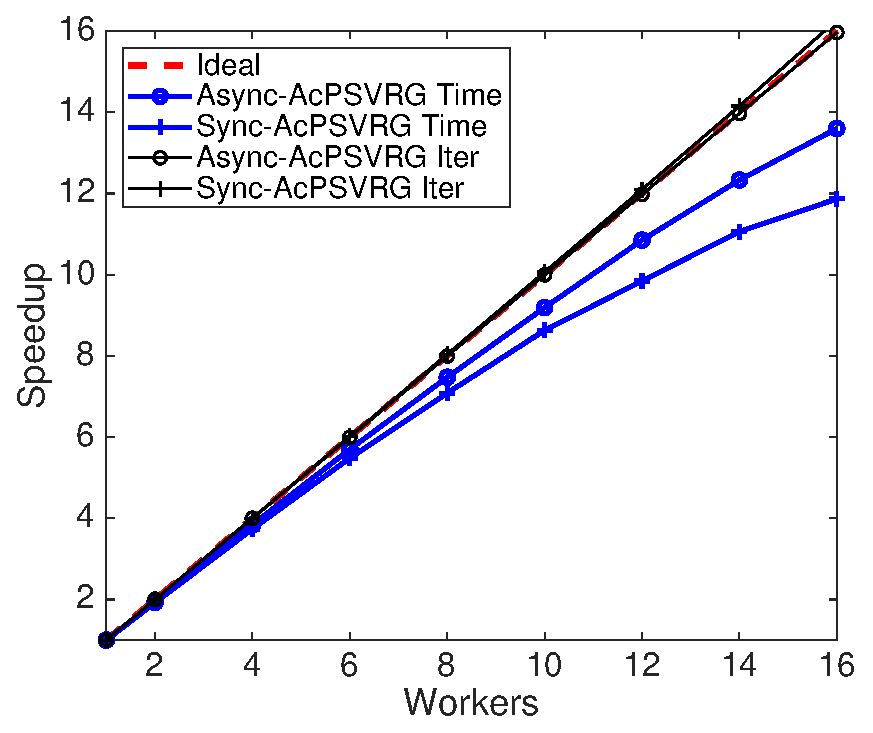
\includegraphics[width=0.24\linewidth]{../Figures/rcv1_speedup_FSVRG.eps}}%
\setlength{\abovecaptionskip}{2pt}
\caption{Scalability analysis of Sync-AcPSVRG and Async-AcPSVRG with iteration and time speedup. }
\label{fig:FSVRG_speedup}
\end{figure*}
We have the following convergence result.
\begin{theorem}\label{conve-theorem}
Suppose the assumptions of Lemma \ref{lemma1} and further, $\beta_s$ and $\eta$ are chosen such that $\beta_s\leq \frac{1}{s+2}$,  $\lambda_s/\beta_s^2 \leq 1/\beta_{s-1}^2$ and $\eta < \min\{\frac{1}{4L
\tau}, \frac{1}{3L}\}$. 
Then, we have
\begin{equation}
\begin{split}
{\E[F(\widetilde{x}^S)-F(x^*)]}&\leq \frac{1}{\beta_{0}^2(S+2)^2}[F(\widetilde{x}^{0})-F(x^*)] \\ 
&~~~ + {\frac{1}{\eta m_{1}(S+2)^2}}\E[\norm{z_{0}^1-x_*}^2].
\end{split}
\end{equation}
If function $F(x)$ is strongly convex with parameter $\mu$, and $\eta$, $\beta_s$ and $m_s$ are chosen such that $\alpha_s\leq \beta_s/4$ and
\[
\lambda_s' := \lambda_s+{\frac{2 \beta_s^2}{\mu\eta m_s}} < 1,
\]
we have, 
\begin{equation}
\E\left[F(\widetilde{x}^S)-F(x^*)\right]\leq \lambda_{max}^S\left[F(\widetilde{x}^0)-F(x^*)\right],
\end{equation}
where $\lambda_{max} = \max_{s}{\lambda_s'}$.
\end{theorem}
\begin{proof}
By selecting $\eta < \min\{\frac{1}{4L
\tau}, \frac{1}{3L}\}$, we have $\alpha_s\leq \frac{1}{2}$. From Lemma \ref{lemma1} we have,
\begin{equation}
\begin{split}
\E[F(\widetilde{x}^s)&-F(x^*)]\leq  \lambda_s[F({\widetilde x}^{s-1})-F(x^*)]\\ 
&+ {\frac{\beta_s^2}{2\eta m_s(1-\alpha_s)}}\E[\norm{z_{0}^s-x_*}^2-\norm{z_{m_s}^s-x_*}^2].
\end{split}
\end{equation}
Dividing both sides of the above inequality by $\beta_s^2$, and using the fact $\lambda_s/\beta_s^2 \leq 1/\beta_{s-1}^2$ we have
\begin{equation*}
\begin{split}
\frac{\E[F(\widetilde{x}^s)-F(x^*)]}{\beta_s^2}&\leq  \frac{\lambda_s}{\beta_s^2}[F(\widetilde{x}^{s-1})-F(x^*)]\\ 
& + {\frac{1 }{2\eta m_s(1-\alpha_s)}}\E[\norm{z_{0}^s-x^*}^2-\norm{z_{m_s}^s-x^*}^2]\\
\stackrel{a}{\leq} & \frac{1}{\beta_{s-1}^2}[F(\widetilde{x}^{s-1})-F(x^*)] \\
&+ {\frac{1}{2\eta m_s(1-\alpha_s)}}\E[\norm{z_{0}^s-x^*}^2-\norm{z_{m_s}^s-x^*}^2], 
\end{split}
\end{equation*}
where in inequality $\stackrel{a}{\leq}$ we used $\frac{\lambda_s}{\beta_s^2}\leq \frac{1}{\beta_{s-1}^2}$. By using $z_0^{s+1} = z_{m_s}^s$, and adding the above inequality from $s=1$ to $S$, we have
\begin{equation*}
\begin{split}
\frac{\E[F(\widetilde{x}^S)-F(x^*)]}{\beta_S^2}\leq & \frac{1}{\beta_{0}^2}[F(\widetilde{x}^{0})-F(x^*)] + {\frac{1}{\eta m_0}}\E\left[\norm{z_{0}^1-x_*}^2\right], \\
\end{split}
\end{equation*}
where we used $m_1\leq m_s$ and $\alpha_s\leq \frac{1}{2}$.
Then we have
\begin{equation*}
\begin{split}
~~~\E[& F(\widetilde{x}^S)-F(x^*)]\\
\leq & \frac{\beta_S^2}{\beta_{0}^2}[F(\widetilde{x}^{0})-F(x^*)]+ {\frac{ \beta_S^2}{\eta m_1}}\E[\norm{z_{0}^1-x_*}^2\\
\leq & \frac{1}{\beta_{0}^2(S+2)^2}[F(\widetilde{x}^{0})-F(x^*)] + {\frac{1 }{\eta m_1(S+2)^2}}\E[\norm{z_{0}^1-x_*}^2].
\end{split}
\end{equation*}

Now suppose $F(x)$ is $\mu$-strongly convex. Since $x^*$ is the optimal solution, by inequality \eqref{Convex:Eq1} we have 
\begin{equation}\label{Eq1-Theo1}
\nabla F(x^*) = 0,\qquad F(x)-F(x^*) \geq \frac{\mu}{2} \norm{x-x^*}^2.
\end{equation}
Using the inequality in \eqref{Eq1-Theo1} and $z_0^s = \widetilde{x}^{s-1}$, we have 

\begin{equation}
\begin{split}
&\E [F(\widetilde{x}^s)-F(x^*)]\\
&\stackrel{a}{\leq}\lambda_s\E[F(\widetilde{x}^{s-1})-F(x^*)]\\
&~~~+ {\frac{ \beta_s^2}{2 m_s\eta(1-\alpha_s)}}\E[\norm{z_{0}^s-x_*}^2-\norm{z_{m}^s-x_*}^2]\\
&\stackrel{b}{\leq}\lambda_s\E[F(\widetilde{x}^{s-1})-F(x^*)]+ {\frac{2  \beta_s^2}{\mu\eta m_s}}\E[F(\widetilde{x}^{s-1})-F(x^*)]\\
&=(\lambda_s+{\frac{2  \beta_s^2}{\mu\eta m_s}})\E[F(\widetilde{x}^{s-1})-F(x^*)],
\end{split}
\end{equation}\\
where the inequality $\stackrel{a}{\leq}$ follows from Lemma \ref{lemma1}, and $\stackrel{b}{\leq}$ is due to the inequality \eqref{Eq1-Theo1} and the inequality $\alpha_s\leq \frac{1}{2}$. 
\end{proof}
As a corollary, we immediately obtain an expected linear rate of convergence for the synchronous algorithm Sync-AcPSVRG for the strongly convex case.
\begin{corollary}\label{cor-syn}
Suppose function $F$ is strongly convex and $\beta_s$, $m_s$ and step size $\eta$ are chosen
such that the following condition is satisfied
\[
\lambda_s' := 1-\beta_s+{\frac{2\beta_s^2}{\eta\mu m_s}} < 1,
\]
Then, for iterates of algorithm Sync-AcPSVRG, we have
\begin{equation}
\E\left[F(\widetilde{x}^S)-F(x^*)\right]\leq \lambda_{max}^S\left[F(\widetilde{x}^0)-F(x^*)\right], 
\end{equation}
with $\lambda_{max} = \max_{s}{\lambda_s'}$. The optimal value of $\lambda$ is $\lambda_{max} = 1-\frac{\mu m_s\eta}{8}$ which is obtained by choosing ${\beta_s=\frac{\mu m_s\eta}{4}}$.
\end{corollary}
\begin{proof}
For the synchronous algorithm, $\tau=0$, and consequently $\alpha_s=0$. Then, from Theorem \ref{conve-theorem}, we have $\lambda_s = 1-\beta_s$ and 
\[
\lambda_s' = 1-\beta_s+{\frac{2  \beta_s^2}{\mu\eta m_s}}.\]
The minimal value of $\lambda_{max}$ is obtained by minimizing $\lambda_s'$ with respect to $\beta_s$.
\end{proof}

\begin{remark}
Compared to Sync-AcPSVRG, due to the delay the convergence rate for Async-AcPSVRG is slower and thereby we prove an asynchronous speedup. In order to obtain speedup for Async-AcPSVRG, the order of inner loop $m_s$ cannot be $\tau$ times larger than Async-AcPSVRG. From Corollary \ref{cor-syn} for Sync-AcPSVRG, the inner loop size in the order of $\mathcal{O}(L/\mu)$ makes $\lambda'_s<1$. In Theorem \ref{conve-theorem}, the condition $\lambda_s/\beta_s^2 \leq 1/\beta_{s-1}^2$ can be satisfied by choosing $\beta_{s-1}/\sqrt{2}\leq \beta_s < \beta_{s-1}$. Further, for inequality $\alpha_s\leq \beta_s/4$, it is sufficient to have 
\begin{equation}
\begin{split}
\eta \leq \frac{\sqrt{\beta_s}}{4L\tau}
\end{split}
\end{equation}
where we use  $\theta_\eta^{-1} \leq 1$ which is from $\eta< \frac{1}{3L}$.
Hence from Theorem \ref{conve-theorem}, the step size $\eta_s$ satisfies $\eta_s<\min\{\frac{\sqrt{\beta_s}}{4L\tau},\frac{1}{4L
\tau}, \frac{1}{3L}\}$. By having $\lambda_s'<1$, we obtain 
\begin{equation}
\begin{split}
\frac{16(1-\alpha_s)L\tau\sqrt{\beta_s}}{\mu} \leq m_s.
\end{split}
\end{equation}
Thus, by setting $\sqrt{\beta_s}\leq \frac{1}{\tau}$ the inner loop size $m_s$ should be $\mathcal{O}(L/\mu)$ to make $\lambda_s'<1$ which is the same as Sync-AcPSVRG. Therefore, one we can achieve linear speedup for Async-AcPSVRG using adaptive step sizes.
\end{remark}
\begin{corollary}\label{cor-asyn}
Suppose function $F$ is strongly convex and 
let $\eta_s=\frac{\sqrt{\beta_s}}{4L\tau}$, $\beta_s< \min\{\frac{1}{\tau^2},\frac{1}{s+2}\}$, and $m_s=\frac{32L}{\mu}$, then, 
\[
\lambda_s' := \lambda_s+{\frac{2 \beta_s^2}{\mu\eta m_s}} < 1-\frac{\beta_s}{2},
\]
and for iterates of algorithm Async-AcPSVRG, we have
\begin{equation}
\E\left[F(\widetilde{x}^S)-F(x^*)\right]\leq \lambda_{max}^S\left[F(\widetilde{x}^0)-F(x^*)\right], 
\end{equation}
with $\lambda_{max} = \max_{s}{\lambda_s'}$. 
\end{corollary}
\begin{remark}
For convex functions, we set $\eta=\frac{1}{5L\tau}$, the number of epochs $S$ is in the same order of $\mathcal{O}(\sqrt{\frac{L\tau}{m}}\frac{1}{\sqrt{\epsilon}})$.
Compared with Sync-AcPSVRG, it
is at most $\sqrt{\tau}$ larger but the computing time is $\tau$ times smaller.
The computation can be distributed to multiple
workers to get $\tau$ times speedup which is in proportion to the number of local workers $P$. Hence, Async-AcPSVRG can
obtain at least $\sqrt{P}$ times speedup.
\end{remark}
\section{Experiments}
%









\begin{table}[htbp]
\begin{center}
\caption{Summary of training datasets.}
\begin{tabular}{ c|c|c|c } 
 \hline
 Datasets &  Data & Features & Non-zeros \\ 
 \hline
  ijcnn & 35,000 & 22 &  455,000\\
  covtype & 581,012 & 54 & 7,521,450\\ 
 %w8a & 49,749  & 300 & 2 \\ 
 real-sim &  72,309 & 20,958 &  3,709,083 \\
 rcv1 & 20,242 & 47,236 &  50,233,657\\
%  \hline
% SUSY & 5,000,000 & 18 &  88,938,127 \\
 %epsilon &  400,000 & 2,000 &  800,000,000 \\
 %kdd12 & 119,705,032 & 54,686,452 & 0 \\
 \hline
\end{tabular}
\label{metadata}
\end{center}
\end{table}
\begin{figure*}[htbp]

\subfigure[comparison on ijcnn]{
\centering
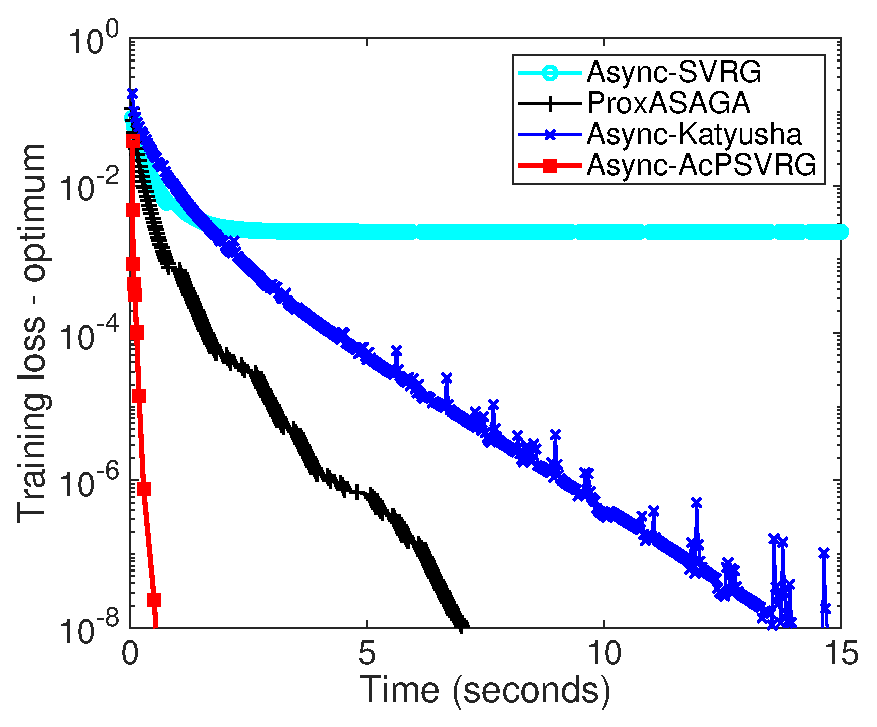
\includegraphics[width=0.24\linewidth]{../Figures/ijcnn_obj_dev_comparison_time.eps}}%
\subfigure[comparison on covtype]{
\centering
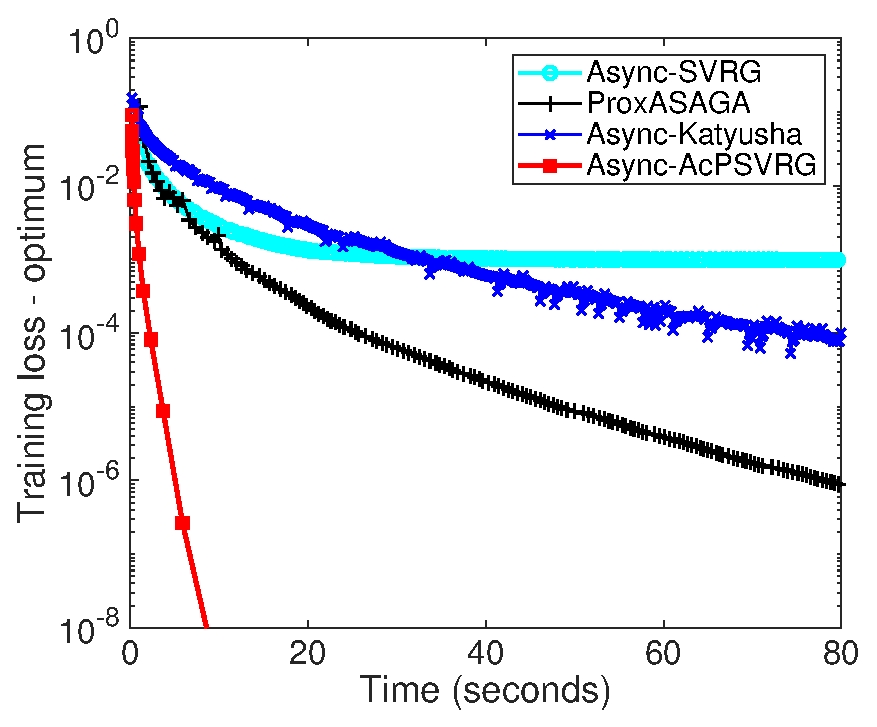
\includegraphics[width=0.24\linewidth]{../Figures/covtype_obj_dev_comparison_time.eps}}%
\subfigure[comparison on real-sim]{
\centering
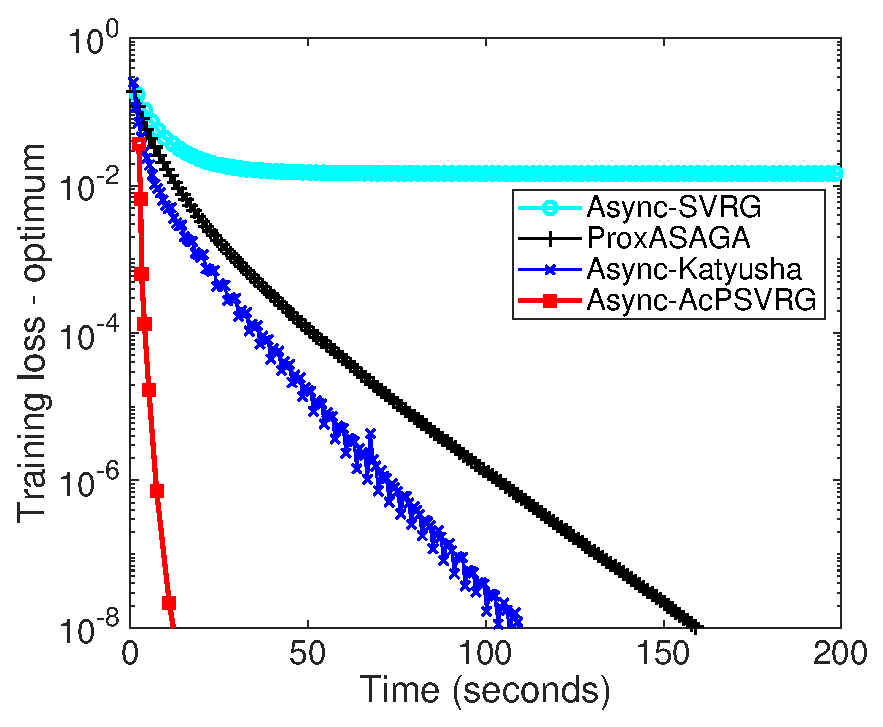
\includegraphics[width=0.24\linewidth]{../Figures/real-sim_obj_dev_comparison_time.eps}}%
\subfigure[comparison on rcv1]{
\centering
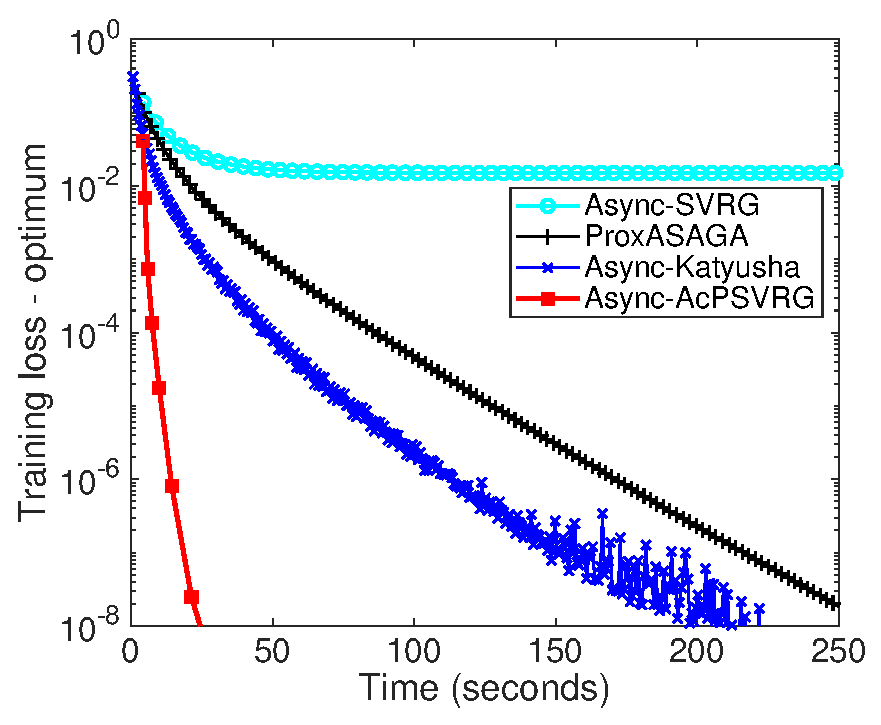
\includegraphics[width=0.24\linewidth]{../Figures/rcv1_obj_dev_comparison_time.eps}}%
\setlength{\abovecaptionskip}{2pt}
\caption{Training loss residual $f(x) - f(x^*)$ versus time plot of Async-SVRG, ProxASAGA, Async-Katyusha, and Async-AcPSVRG. }
\label{fig:algo_comp}
\end{figure*}
We present our empirical results in this section. For our experiments, we study logistic regression loss function with $L_2$ regularization. The problem can be formulated as optimization problem \eqref{problem} with $f_i(x) = \log(1+e^{-y_iz^T_i{x}})$, $h(x) = \frac{\nu}{2}\|{x}\|^2$, where $z_i\in\R^d$ and $y_i$ is the corresponding label for each $i$. Further, the $L_2$ regularization weight $\nu$ is set $10^{-4}$ in all experiments. We evaluate the following state-of-the-art variance reduction algorithms for our experiments: 1) SVRG \cite{Johnson12}, 2) ProxASAGA \cite{pedregosa2017breaking} and 3) Katyusha \cite{Allen-Zhu17}. The learning rates are tuned for these algorithms in our experiments, and the results shown in this section are based on the best learning rate for each algorithm we achieved.


All the algorithms were implemented in C++ and OpenMPI{\footnote{All simulations were performed on Amazon EC2 t2.large instances with 8 GB RAM.}}. We run our experiments on datasets from LIBSVM website{\footnote{https://www.csie.ntu.edu.tw/~cjlin/libsvmtools/datasets/binary.html}}, as shown in Table \ref{metadata} . The epoch size $m_1$ initially is chosen as 125 in all our experiments and it grows in each epoch by a constant of $\gamma$ = 1.5. In AcPSVRG, we set step sizes $\eta$ and $\beta_s$ to satisfy our assumptions in lemmas and theorems with $\tau\sim P$, where $P$ is the number of workers.

In the first experiment, we compare the speedup achieved by our synchronous and asynchronous algorithm. To this
end, for each dataset we first measure the time required for the algorithm to reach the accuracy of $10^{-10}$. The iteration speedup with $P$ processes is defined as 
\[
 \text{iteration speedup} = \frac{\text{number of iterations with single worker}}{\text{avg. number of iterations with $P$ workers}} \]
and the time speedup is defined as 
 \[
  \text{time speedup} = \frac{\text{runtime with single worker}}{\text{runtime with $P$ workers}}.
\]
%\begin{figure}[htbp]
%\centerline{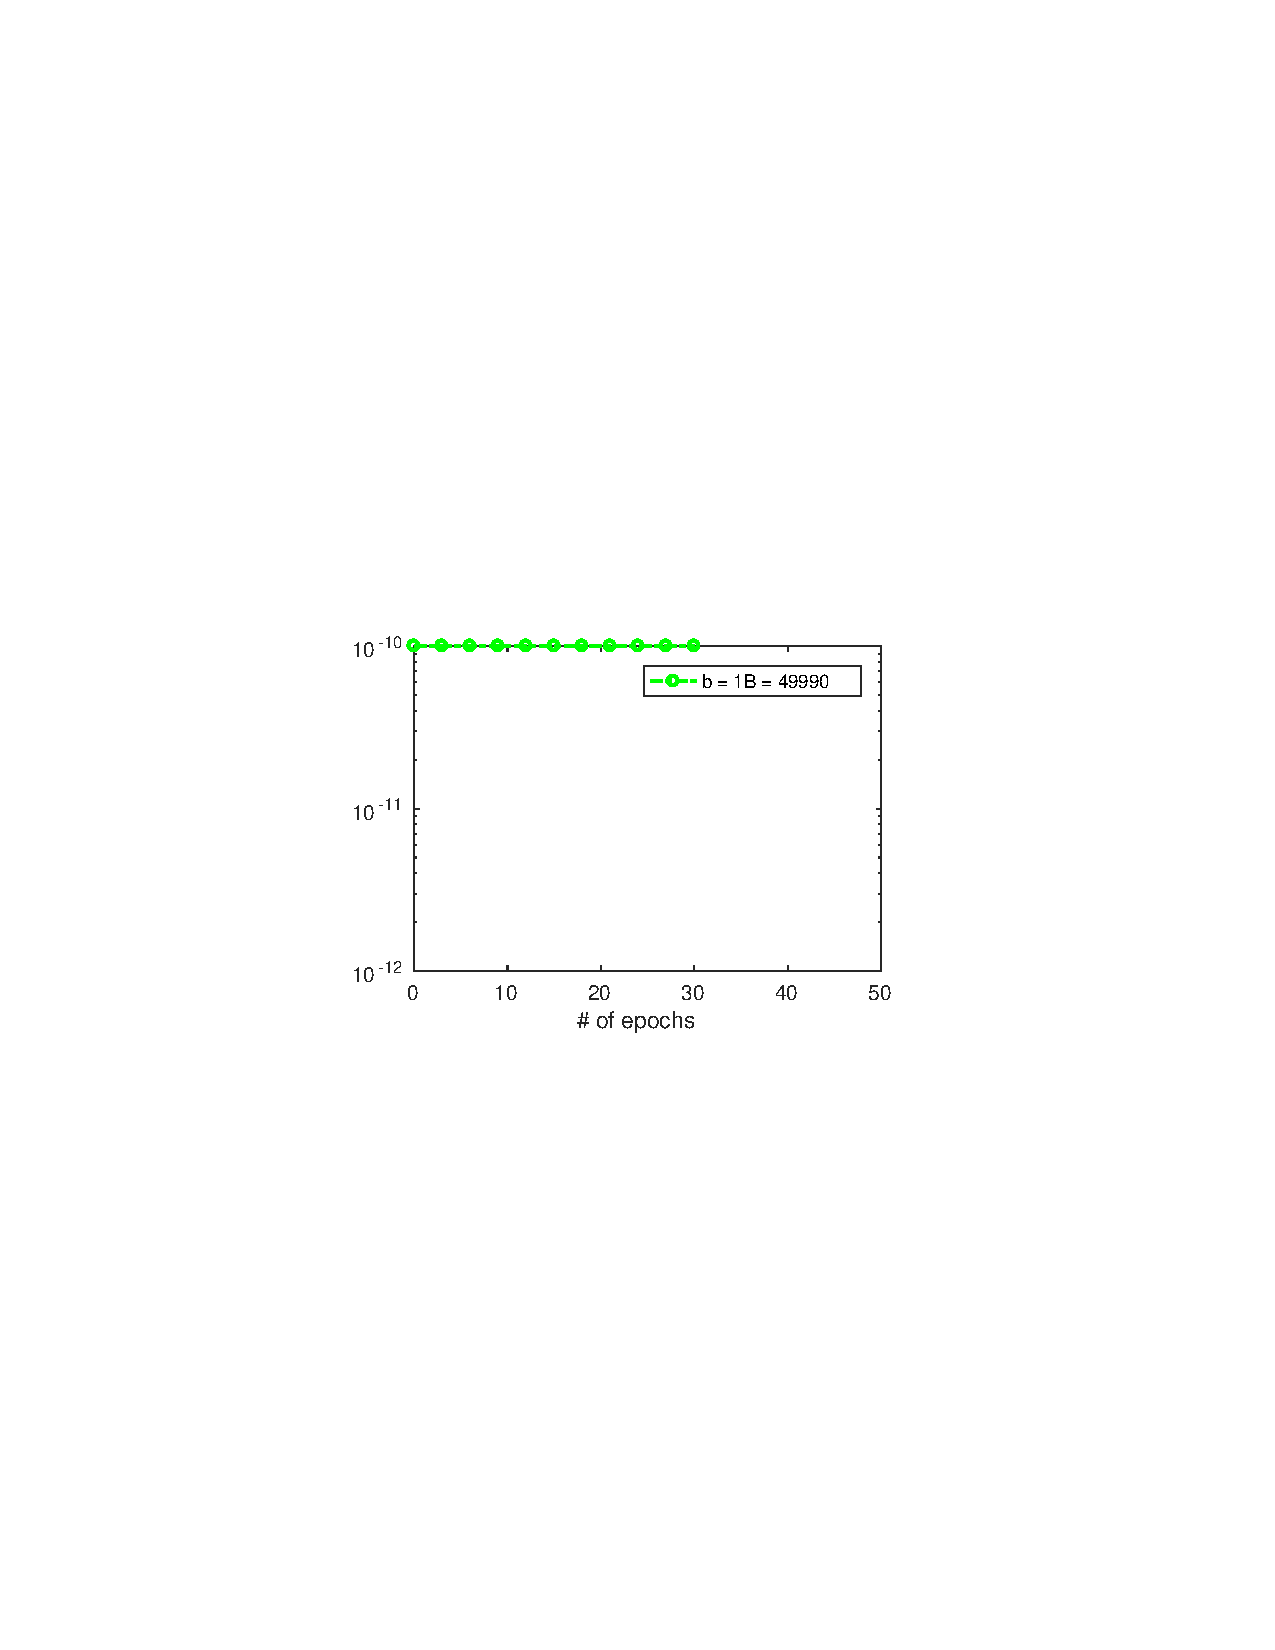
\includegraphics{fig1.png}}
%\caption{Example of a figure caption.}
%\label{fig}
%\end{figure}


Results in Figure \eqref{fig:FSVRG_speedup} show the speedup on various datasets. As shown by Figure \eqref{fig:FSVRG_speedup}, we achieve remarkable speedup for all the datasets. Both synchronous and asynchronous versions show linear iteration speedup in all data sets. Furthermore, the highest
time speedup for Async-AcPSVRG is achieved for ijcnn dataset which has the fewest number of features compared to other datasets we considered in this experiment. Evidently, the time speedup achieved by Async-AcPSVRG is higher than the ones obtained by Sync-AcPSVRG. The speedup for Sync-AcPSVRG improves with the size of datasets, since the synchronization cost, which includes both communication time and waiting time, is dominant compared to computation time on small datasets. The results for Async-AcPSVRG show better scalability compared with \cite{Reddi2015,Meng2016}.



For the second set of experiments we compare the performance of AcPSVRG with the variants of variance reduction stochastic gradient descent described earlier in this section.  
We use 16 workers to compare the algorithms in this experiment. Since the computation complexity of each epoch of these
algorithms is different, in Figure \ref{fig:algo_comp} we directly plot the objective value versus the runtime for each of these algorithms. 
As seen in the figure, Async-AcPSVRG outperforms variance-reduced ProxSGD algorithms in all the cases. In particular compared to Async-Katyusha, as AcPSVRG uses only one auxiliary variable for calculation of momentum, it has lower complexity per iteration and so shows better convergence speed. 
Our proposed algorithms outperform Katyusha in several aspects. First, the plots of Async-Katyusha in asynchronous experiments show much more oscillations compared to our algorithms. This appearance
is caused by the sensitivity of Katyusha  to delayed gradients when calculating momentum terms with local partial data, which introduces variance in training process. Our algorithms do not show sensitivity on delayed gradients. Secondly, AcPSVRG needs to tune only one parameter for momentum acceleration for different datasets while Katyusha needs adjustment of two acceleration parameters in order to achieve a comparable level of performance.

\iffalse
\begin{table}
\begin{center}
\caption{Parameter setting for algorithm implementation. Lmax denotes Lipschitz constant, n is the number of data, and $\rho$ and  $m_s$ are specified to 1.25 and n/4. }
\begin{tabular}{ c|c|c|c } 
 \hline
 Algorithms & initial $\eta$ & Inner Loops & $\lambda$  \\ 
 \hline
 SVRG & 1/(10*Lmax) & 2n & 1e-4\\
 SAGA & 1/(10*Lmax) & n & 1e-4\\
 %SVRG++ & 1/(7*Lmax) & 2n \\ 
 %SVRG-Prox & 1/(7*Lmax) & 2n \\
 Katyusha & Lmax & 2n & 1e-4 \\
 AcPSVRG & 1.5/Lmax &  $\lceil{\rho\cdot m_s}\rceil$ & 1e-4\\
 \hline
\end{tabular}
\label{par_setting}
\end{center}
\end{table}
\fi











\section{Conclusion}
In this paper, we have studied the distributed proximal stochastic gradient algorithms by integrating with variance reduction and momentum acceleration techniques. Using momentum acceleration rate, we have proved their convergence rates, discussed their speedups, and empirically verified our theoretical findings. Our distributed proximal algorithms can achieve nearly linear speedup. The proposed algorithms can reduce the communication cost significantly by increasing the length of epoch by a constant after each epoch. As for future work, we will extend the study in this paper to the non-convex case, and investigate AcPSVRG in shared memory architectures, both theoretically and empirically.


%\bibliography{GTA}
\bibliography{VarianceReductionAAAI}
\bibliographystyle{aaai}
\end{document}
